%% BioMed_Central_Tex_Template_v1.06
%%                                      %
%  bmc_article.tex            ver: 1.06 %
%                                       %

%%IMPORTANT: do not delete the first line of this template %It must be present
%to enable the BMC Submission system to %recognise this template!!

%%%%%%%%%%%%%%%%%%%%%%%%%%%%%%%%%%%%%%%%%
%%                                     %%
%%  LaTeX template for BioMed Central  %% %     journal article submissions
%%%
%%                                     %%
%%          <8 June 2012>              %%
%%                                     %%
%%                                     %%
%%%%%%%%%%%%%%%%%%%%%%%%%%%%%%%%%%%%%%%%%

%%%%%%%%%%%%%%%%%%%%%%%%%%%%%%%%%%%%%%%%%%%%%%%%%%%%%%%%%%%%%%%%%%%%%
%%                                                                 %%
%% For instructions on how to fill out this Tex template           %% % document
%please refer to Readme.html and the instructions for   %% % authors page on the
%biomed central website                      %% %
%http://www.biomedcentral.com/info/authors/                      %%
%%                                                                 %%
%% Please do not use \input{...} to include other tex files.       %% % Submit
%your LaTeX manuscript as one .tex document.              %%
%%                                                                 %%
%% All additional figures and files should be attached             %% %
%separately and not embedded in the \TeX\ document itself.       %%
%%                                                                 %%
%% BioMed Central currently use the MikTex distribution of         %% % TeX for
%Windows) of TeX and LaTeX.  This is available from      %% %
%http://www.miktex.org                                           %%
%%                                                                 %%
%%%%%%%%%%%%%%%%%%%%%%%%%%%%%%%%%%%%%%%%%%%%%%%%%%%%%%%%%%%%%%%%%%%%%

%%% additional documentclass options: [doublespacing] [linenumbers]   - put the
%  line numbers on margins

%%% loading packages, author definitions

%\documentclass[twocolumn]{bmcart}% uncomment this for twocolumn layout and
%comment line below
\documentclass{bmcart}

%%% Load packages \usepackage{amsthm,amsmath} \RequirePackage{natbib}
%\RequirePackage[authoryear]{natbib}% uncomment this for author-year
%bibliography \RequirePackage{hyperref}
\usepackage[utf8]{inputenc} %unicode support
%\usepackage[applemac]{inputenc} %applemac support if unicode package fails
%\usepackage[latin1]{inputenc} %UNIX support if unicode package fails
\usepackage{graphicx}
\usepackage{placeins}
\usepackage{subcaption}
\usepackage{amsthm,amsmath}

%%%%%%%%%%%%%%%%%%%%%%%%%%%%%%%%%%%%%%%%%%%%%%%%%
%%                                             %%
%%  If you wish to display your graphics for   %% %  your own use using
%includegraphic or       %% %  includegraphics, then comment out the      %% %
%following two lines of code.               %% %  NB: These line *must* be
%included when     %% %  submitting to BMC.                         %% %  All
%figure files must be submitted as      %% %  separate graphics through the BMC
%%% %  submission process, not included in the    %% %  submitted article.
%%%
%%                                             %%
%%%%%%%%%%%%%%%%%%%%%%%%%%%%%%%%%%%%%%%%%%%%%%%%%

% \def\includegraphic{} \def\includegraphics{}

%%% Put your definitions there:
\startlocaldefs
\endlocaldefs

%%% Begin ...
\begin{document}

%%% Start of article front matter
\begin{frontmatter}

\begin{fmbox}
\dochead{Research}

%%%%%%%%%%%%%%%%%%%%%%%%%%%%%%%%%%%%%%%%%%%%%%
%%                                          %%
%% Enter the title of your article here     %%
%%                                          %%
%%%%%%%%%%%%%%%%%%%%%%%%%%%%%%%%%%%%%%%%%%%%%%

\title{The developement of a smart way for monitoring patients' vital signs}

%%%%%%%%%%%%%%%%%%%%%%%%%%%%%%%%%%%%%%%%%%%%%%
%%                                          %%
%% Enter the authors here                   %%
%%                                          %%
%% Specify information, if available,       %% % in the form: %% %
%<key>={<id1>,<id2>}                    %% %   <key>= %% % Comment or delete the
%keys which are     %% % not used. Repeat \author command as much %% % as
%required.                             %%
%%                                          %%
%%%%%%%%%%%%%%%%%%%%%%%%%%%%%%%%%%%%%%%%%%%%%%

\author[ addressref={aff1}, email={michael187107@fci.bu.edu.eg}
]{\inits{MGR}\fnm{Michael G} \snm{Rizk}}

\author[ addressref={aff1}, email={samaa187070@fci.bu.edu.eg}
   ]{\inits{STE}\fnm{Samaa T} \snm{El Sersy}}

   \author[ addressref={aff1}, email={ismail187006@fci.bu.edu.eg}
   ]{\inits{IMH}\fnm{Ismail M} \snm{Helal}}

\author[ addressref={aff1}, email={youssef187167@fci.bu.edu.eg}
]{\inits{YAA}\fnm{Youssouf A} \snm{Ahmed}}

\author[ addressref={aff1}, email={mohamed187109@fci.bu.edu.eg}
]{\inits{MER}\fnm{Mohammed E} \snm{Rashad}}

%%%%%%%%%%%%%%%%%%%%%%%%%%%%%%%%%%%%%%%%%%%%%%
%%                                          %%
%% Enter the authors' addresses here        %%
%%                                          %%
%% Repeat \address commands as much as      %% % required.
%%%
%%                                          %%
%%%%%%%%%%%%%%%%%%%%%%%%%%%%%%%%%%%%%%%%%%%%%%

\address[id=aff1]{%                           % unique id
  \orgname{Department of Medical Informatics, Benha}, % university, etc
  \street{Fareed Nada Street},                     %
  %\postcode{}                                % post or zip code
  \city{Benha},                              % city
  \cny{EG}                                    % country
} 

%%%%%%%%%%%%%%%%%%%%%%%%%%%%%%%%%%%%%%%%%%%%%%
%%                                          %%
%% Enter short notes here                   %%
%%                                          %%
%% Short notes will be after addresses      %% % on first page.
%%%
%%                                          %%
%%%%%%%%%%%%%%%%%%%%%%%%%%%%%%%%%%%%%%%%%%%%%%

% \begin{artnotes} %\note{Sample of title note}     % note to the article
% \note[id=n1]{Equal contributor} % note, connected to author \end{artnotes}

\end{fmbox}% comment this for two column layout

%%%%%%%%%%%%%%%%%%%%%%%%%%%%%%%%%%%%%%%%%%%%%%
%%                                          %%
%% The Abstract begins here                 %%
%%                                          %%
%% Please refer to the Instructions for     %% % authors on
%http://www.biomedcentral.com  %% % and include the section headings         %%
%% accordingly for your article type.       %%
%%                                          %%
%%%%%%%%%%%%%%%%%%%%%%%%%%%%%%%%%%%%%%%%%%%%%%

\begin{abstractbox}
\begin{abstract} % abstract
\parttitle{Background} %if any
Health care is an integral part of human life, and due to the huge increase of
people and the increase in diseases, especially cardiovascular diseases and
chronic diseases, it has become difficult for hospitals to accommodate this huge
number of people. The early detection of critical abnormal situations without
the need for direct contact with the patient, so a remote health care system was
proposed that relies on artificial intelligence and advanced computing. This
system was designed to continuously monitor physiological processes such as
heart rate and blood oxygen saturation level, and also detects abnormal
conditions such as arrhythmia or cardiac arrest, and immediately alert the
relevant organizations for the immediate intervention. In this paper, we review
how to use wearable sensing devices for monitoring the physiological processes
of an individual, detect the abnormal conditions such as arrhythmia and cardiac
arrest, and immediately alert the relevant organizations.

\parttitle{Methods} %if any
This paper reviews the methods of estimating heart rate and blood oxygen
saturation in different ways and the data structure, and then the system model
developed to give the user the ability of storing and sharing the data, online
database which allows all the users’ data to be stored online safely and viewing
the data changes in real time in case of real time data, and  lastly cloud
messaging provide the ability to send notifications from device to another in
case of abnormal behavior detected in one of the users’ vital signs, , and
finally testing the performance and accuracy of the developed model.

\parttitle{Keywords} %if any
health care, early detection, vital signs monitoring, ML.

\end{abstract}

%%%%%%%%%%%%%%%%%%%%%%%%%%%%%%%%%%%%%%%%%%%%%%
%%                                          %%
%% The keywords begin here                  %%
%%                                          %%
%% Put each keyword in separate \kwd{}.     %%
%%                                          %%
%%%%%%%%%%%%%%%%%%%%%%%%%%%%%%%%%%%%%%%%%%%%%%

\begin{keyword}
\kwd{sample}
\kwd{article}
\kwd{author}
\end{keyword}

% MSC classifications codes, if any \begin{keyword}[class=AMS] \kwd[Primary ]{}
%\kwd{} \kwd[; secondary ]{} \end{keyword}

\end{abstractbox}
%
%\end{fmbox}% uncomment this for twcolumn layout

\end{frontmatter}

%%%%%%%%%%%%%%%%%%%%%%%%%%%%%%%%%%%%%%%%%%%%%%
%%                                          %%
%% The Main Body begins here                %%
%%                                          %%
%% Please refer to the instructions for     %% % authors on: %% %
%http://www.biomedcentral.com/info/authors%% % and include the section headings
%%% % accordingly for your article type.       %%
%%                                          %%
%% See the Results and Discussion section   %% % for details on how to create
%sub-sections%%
%%                                          %%
%% use \cite{...} to cite references        %% %  \cite{koon} and %% %
%\cite{oreg,khar,zvai,xjon,schn,pond}    %% %
%\nocite{smith,marg,hunn,advi,koha,mouse}%%
%%                                          %%
%%%%%%%%%%%%%%%%%%%%%%%%%%%%%%%%%%%%%%%%%%%%%%

%%%%%%%%%%%%%%%%%%%%%%%%% start of article main body <put your article body
% there>

%%%%%%%%%%%%%%%%
%% Introduction %%
%%
\section*{Introduction}
Quality health care is a basic human right, and unfortunately it is not
adequately provided as a result of the economic, social and environmental change
and subsequent changes in lifestyle to a significant increase in chronic
diseases such as heart disease, and this represents a major threat to human
health and therefore every time an infectious disease spreads Hospitals are
crowded and filled with people, sometimes diseases are linked to changes in some
physiological rates in the human body, such as heart rate and blood oxygen
saturation. Or the severe lack of normal rates is a strong sign of death for a
large number of patients, and because some people cannot go to the hospital from
time to time, they may not have enough time or they have a chronic disease or
the specialist abroad.\\
In addition, health care may cost the hospital a lot for these people.
Therefore, health devices are a reliable solution for monitoring, recording and
tracking vital processes at home. We can also request medical help in case of
emergency. Medical devices have a very great interest and have become very
widespread and commercially available.\\
Remote health care monitoring has become a major concern in our time today, so
specialists are looking for a system that monitors vital processes and provides
accurate diagnoses and suggestions for user health, taking into account the
patient's past and current health conditions.\\
With the many developments that have taken place in the Internet of Things and
wireless sensor networks, many attempts have been made remotely without going to
the hospital, and this helps specialists to determine appropriate procedures in
advance or to send assistance in case of emergency, and the transfer of
important data to the patient may affect his life using cloud computing, Which
is a paradigm shift in computing and cloud storage is where patient data is
stored and processed, allowing patient vital signs to be monitored and stored
for historical reviews.\\
Storing patient data in the cloud provides low cost, convenience, and
reliability, and we also need a way to deliver important patient data to
healthcare providers while taking into account patient privacy.\\
The proposed system provides a very convenient and secure solution for recording
health data stored in the cloud. Biometric sensors are used to remotely measure
key biological markers such as heart rate and blood oxygen saturation for a
person while they are resting at home.\\
This system targets patients with medical problems such as emergency diseases,
accident patients, patients with movement disabilities and chronic diseases, as
well as patients suffering from infectious diseases such as Covid 19 disease,
patients who follow up with doctors abroad, as well as the elderly who need
continuous care.\\
These devices send data wirelessly to the cloud via a mobile phone application,
which makes it easier for doctors to monitor the condition of their patients,
and this allows doctors to follow up on the condition of their patients and make
suggestions accordingly.\\
Machine learning techniques allow a revolution in the digital healthcare sector,
as well as artificial intelligence plays an important, essential and vital role
in remote healthcare monitoring systems for patients based on the Internet of
things to diagnose and prevent diseases in order to maintain the health of
patients, especially cardiovascular patients.\\
Furthermore, sensors create a tremendous volume of data in the IoT environment.
This data contains significant healthcare information; hence it is critical to
study it in order to develop medical technology. AI and ML technology would be
incredibly valuable in this area for doing data analytics, categorization, and
forecasting healthcare issues based on this data.\\
We created and deployed a smart remote monitoring system based on IoT in
response to the pressing requirement for remote patient monitoring and its
benefits. The system records and sends data from several wearable sensors to the
edge device, which leverages edge computing to make choices locally using ML
approaches.\\
The suggested system is a device that uses a distant location to monitor a
patient's vitals, such as oxygen saturation, body temperature, and heart rate.\\
Because the IoT node will create significant volumes of data on a regular basis
from a variety of patients, AI and ML technologies are employed at the edge to
do data analytics, categorization, and prediction of healthcare issues. ML
algorithms extract statistics from raw data to gain insights about the patient's
health.\\
The system provides an application that allows to follow the status of the user.
The application is small, simple, understandable, easy to handle and flexible.
In order to know the health status of the patient or the user, the machine
learning model is trained at the cloud level and then this model is implemented
on the edge device, through which the patient’s health status is predicted based
on the readings.\\

%%%%%%%%%%%%%%%%
%% Related Work %%
%%
\section*{Related Work}
In Asia and Europe, cardiovascular diseases (CVD) are the leading causes of
death; mortality rates are greater among women and patients with poor
socioeconomic level. The system that will monitor patients' vital metrics on a
regular basis and give treatment recommendations based on medical data and
health state is urgently needed [1].\\
Different surveyed articles are examined in this part to evaluate the
performance of digital healthcare systems that have previously been established
and how they contribute to healthcare IoT. One study [2] highlights the
necessity of healthcare monitoring systems for cardiovascular disease and the
need for medical personnel to share data from patients living in remote
locations. This is critical since inhabitants in rural locations are often cut
off from the metropolitan population and have limited access to medical care.\\
The development and design of a wearable electrocardiogram (ECG) monitor using
Arduino are discussed in this article. The system architecture consists of
bio-sensing modules, a cloud (Google Firebase) for storing real-time patient
data, and a web interface for medical experts to view the data and provide rapid
diagnosis and treatment of any developing cardiovascular illness. The study's
main result is the creation of a low-cost, portable, and full real-time ECG
capture, transmission, storage, and display system based on the Internet of
Things. Medical practitioners can use this real-time data to diagnose heart
disorders by   visualizing it. Furthermore, the information is sent into a
diagnostic software with a graphical user interface (GUI). The biggest
disadvantage of this technology is that it may have difficulties with latency
and network access, particularly in remote locations. Our system includes an
edge-based architecture that conducts local anomaly detection based on ML to
deal with crises to handle this essential challenge.\\
The authors of [3] follow a similar approach, emphasising the relevance of ECG
signals in cardiovascular patients. They offer an IoT-based health monitoring
system that observes the underlying data using a statistical model called the
Hidden Markov Model. ECG signal characteristics as collected by a sensor the aim
of this program is to make it easier to get better results. Patients with CVD
will benefit from better monitoring and faster intervention, which will improve
medical care. in the case of such patients A patient path estimator, a patient
path estimator, and a patient path estimator are all used in the system's
implementation.  Within the hospital, there are table and alert management
schemes to help with localization and alarm management. Treatment of CVD
patients should be started as soon as possible. The classification of an ECG
signal is based on the time between each RR peak, as well as the amplitude R
peaks. These are used combined to detect common and significant rhythm problem
peaks. The criteria of RR $>$ 150 ms and t period $>$60 ms are determined based
on comparative data of 50 normal patients and 50 CVD patients, resulting in a
strong positive prediction of CVD. The disadvantage is that this article does
not include the installation of smarter technologies based on AI and machine
learning. As a result, additional modifications are still required to increase
the diagnostic model's accuracy\\
The researchers in [4] believe that advances in machine learning technology have
enabled early illness identification and diagnosis. This is especially
beneficial in the case of chronic ailments, such as heart disease. A bespoke
machine is proposed in this study. In the next ten years, a learning algorithm
will be used to forecast the likelihood of cardiac disease. Hard Voting (HV)
classifier is the name given to their algorithm. HV was created utilizing
logistic Regression, Random Forest, Multilayer Perceptron, and other well-known
classifiers  Nave Bayes classifiers with Gaussian Multiple risk variables (e.g.,
age, gender) are taken into account by the meta-classifier. As inputs, sex,
smoking, systolic blood pressure, and so on. Each of the four classifiers is
employed, and  a vote is taken to determine whose forecast is the best. The
researchers utilized data from 3751 patients from a publicly available dataset
on Kaggle. To eliminate any outliers, the authors utilized RobustScaler to scale
the data. For training and testing purposes, the dataset was separated into two
halves with an 80–20 percent split. The meta-classifier algorithm was
successfully designed, with an accuracy of 88.42 percent and a precision value
of 1.0 on the test. The construction of the ML model is the emphasis of this
work, not any IoT-based ECG monitoring system. The authors did not test their
model using real-time patient data. Not only are numerous vitals collected in
our suggested architecture, but robust techniques are also applied to forecast
the health status of real-time patients.\\
The researchers propose a method based on IoT and machine learning approaches to
handle the issue of remote monitoring in [5]. It integrates an IoT-based sensor
network with Arduino, namely a pulse sensor. On the data collected for heart
ailment categorization, this system additionally incorporates ML classification
algorithms. The Decision Tree method, Random Backwoods classifier, and Support
Vector Machine were all put to the test in this study (SVM). The authors
gathered data from 40 patients and used it to develop the aforementioned
algorithms. It was discovered that SVM has a greater level of accuracy when it
comes to accurately detecting a cardiac condition (an accuracy of 86 percent).
Patients can use the suggested hardware and software system to forecast cardiac
disease in its early stages. Although this technique aids CVD patients, a
diagnosis based just on pulse data does not provide a complete picture of the
patient's health. To increase the performance of the ML model, more sensors must
be added. As a result, we incorporated many vital sign sensors in our suggested
system to monitor the chronic patient's health.\\
Using federated learning on local Edge computing devices, Article [6] presents
another another smart data analytics architecture for e-healthcare applications.
The need of incorporating federated learning into the system architecture stems
from the sensitive medical data obtained through wearable devices being kept
private and secure. The article provides a detailed explanation of the proposed
framework, which is divided into three modules: cloud, edge, and application.
The authors, on the other hand, make no mention of the system's implementation.
The study's major focus was on identifying federated learning on the edge for
e-health system designs in order to provide service quality (quick reaction
time) and security (data security).[7] proposes CAMISA, an AI-powered system for
remote monitoring of COVID-19 patients. The authors created a Wireless Sensor
Network (WSN) device in the form of a smart shirt and nebulizer that is equipped
with several sensors for obtaining a patient's physiological information. A
patient's pulse, SpO2 level, temperature, and breathing rate are all measured by
the system. If any of these metrics surpass their threshold levels,
notifications are sent to the hospital, including the patient's current location
so that he or she can be sent to critical care as soon as possible. . In
addition, the authors have used a neural network model to estimate the
probability of a user contracting a coronavirus. The Artificial Neural Network
(ANN) model takes 20 characteristics into account, such as the existence of a
cold, fever, or cough, which are all indicators of coronavirus infection. The
health monitoring app collects these parameters from the user via a
questionnaire and determines whether or not the patient has COVID-19. Using the
Thingspeak IoT platform, the app also visualises the sensor data from the
system. This device may be used to remotely monitor COVID-19 patients in real
time to help hospitals curb the virus's spread.

\section*{Methodology}
The proposed method revolves around developing a system with the capability of
monitoring patients’ data using smart phone with the aid of either the phone
camera and AI or a Bluetooth enabled oximeter and phone Bluetooth , then
detecting abnormalities considering the processing ability of the modern smart
phones combined with the cloud services to give each user the ability of storing
and sharing the data, adding other users as connections and notifying other
connections in the case of detecting abnormalities forming an IoT solution for
remote patient health monitoring system that can be adopted as family-oriented
or professional structure.\\
The mobile application developed to connect and receive the data from the
Bluetooth enabled oximeter, making use of the phone camera and flash to estimate
the heart rate and blood oxygen saturation, show the final result for the user.
Besides, opening the gate to the web services giving the ability to connect to
one of the web services SDKs for online collaborative and secure experience.\\
The Bluetooth enabled oximeter circuit consist of 3 main components, first the
biosensor module MAX30102 for heart rate and blood oxygen saturation continues
monitoring [A], second the Bluetooth interface HC-05 interface for data
interfacing between the circuit and the smart phone, and the micro-controller
Arduino UNO (REV3) for all the calculations and the other other components
integration.\\
The mobile camera vital measurement can be divided into three operations, first
getting the signal by recording a video of the users’ fingertip when places on
the camera and flash simultaneously for a period of time and converting the
signal to a form can be used later, second the recoded signal passed to a ML
model to estimate the blood oxygen saturation value and finally the same signal
used again in different calculation discussed later to estimate the heart rate
value.\\
The web services related to all the online features needed such as
authentication to  guarantee each user retain all the data in one single safe
account, online database which allows all the users’ data to be stored online
safely and sharing the data to the permitted users and viewing the data changes
in real time in case of real time data, and  lastly cloud messaging provide the
ability to send notifications from device to another in case of abnormal
behavior detected in one of the user’s vital signs.\\

\subsection*{Circuit Design}
The circuit design shown in Figure 1 illustrates the Bluetooth enables oximeter
circuit used which consists of,  Arduino Uno controller which responsible for
all the calculations, decision making and the whole circuit integration, also
acts as a power supply for the other components, MAX30102 sensor by MAXIM
capable of taking reading of the vital signs with minimum margin of error with
adequate size and power consumption, and  HC-05 Bluetooth transceiver which
allow delivery of vital signs to the mobile device.

\begin{figure}[h!]
  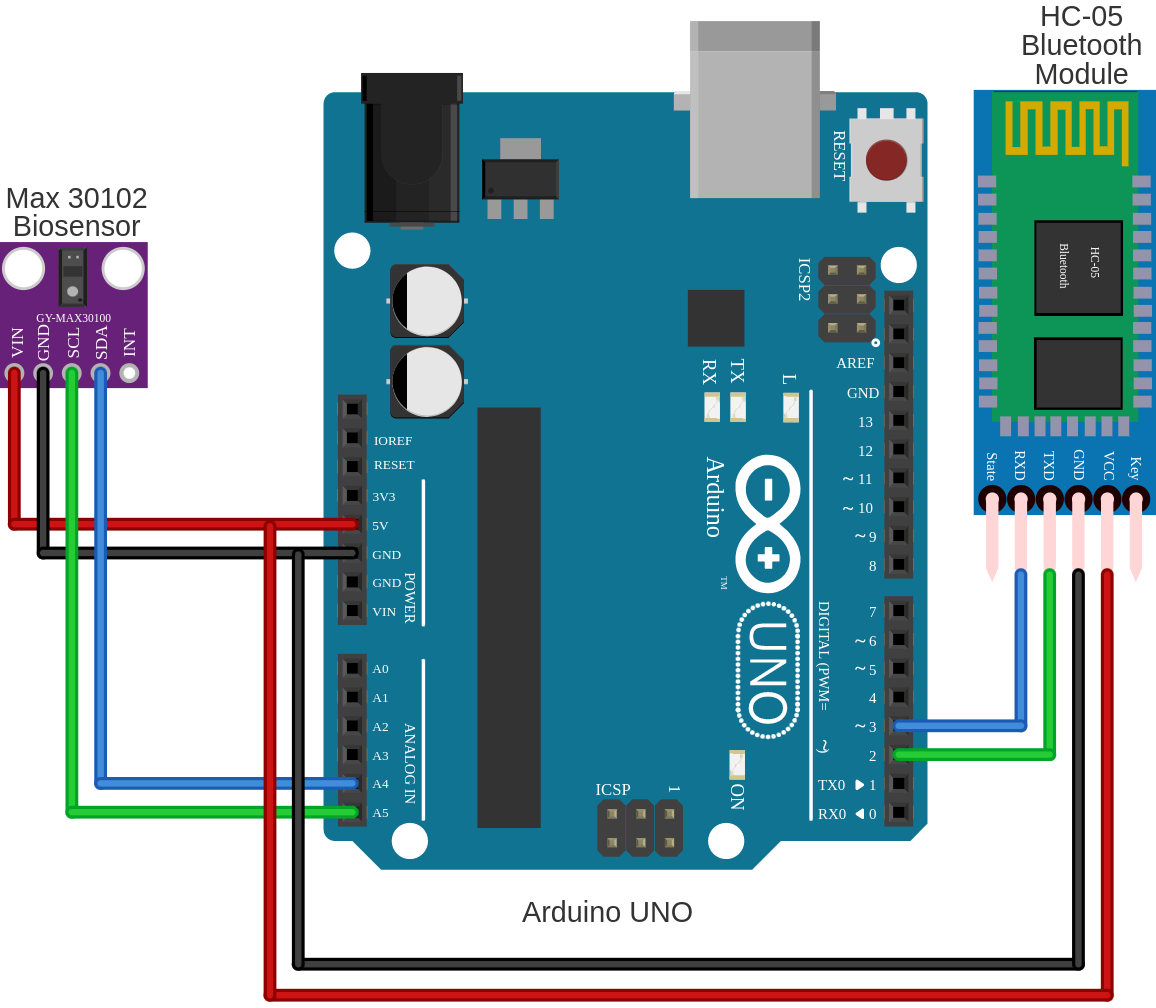
\includegraphics[width=.75\linewidth]{png_images/circuit_desing.png}
  \caption{\csentence{Bluetooth enabled oximeter circuit design.}
      }o
\end{figure}
\FloatBarrier

\subsubsection*{Signal Acquisition}
A typical design will drive the red and IR and LEDs alternately to capture all
the reflected light from the placed finger with the embedded photo-diode then
sent to the controller for further processing.\\

\subsubsection*{Heart Rate Measurement}
The process takes the advantage of the changing level of the light absorption of
the skin associated with blood flow due to the increase of blood volume causing
a brief expansion of the blood vessel as each heartbeat pushed through them
leading to a noticeable peak in the photo-diode readings and by detecting the
time for each peak the heart rate can be calculated according to Equation 1.\\
%
\[
 Heart Rate = \frac{60,000}{Current Peak Timestamp - Previous Peak Timestamp}
 \tag{1}
\]
%

\subsubsection*{Blood Oxygen Measurement}
The process also takes the advantage of  the changing levels different light
absorption of the blood, but unlike the heart rate the process depends on the
different absorption of light found in the hemoglobin in the oxygenated and
deoxygenated states as show in Fig 3.2, Deoxygenated hemoglobin (Hb) absorbs
more light red than infrared light, while oxygenated hemoglobin (HbO2) absorbs
more infrared light than red light by and with information in mind Eq.(2) is
applied, since the final value requires empirical calibration between the ration
and the final spo2 Eq.(3) is applied which proposed by MAXIM%
% TODO: put the figure and add the equtaion labels
%
\[
 Ratio = \frac{AC_r/DC_r}{AC_{ir}/DC_{ir}}
 \tag{2}
\]
\[
 Blood Oxygen = (-45.06 \times Ratio + 30.354) \times Ratio + 94.845
 \tag{3}
\]
%
\cite{koon,khar,zvai,xjon,marg}.
%\nocite{oreg,schn,pond,smith,marg,hunn,advi,koha,mouse}

\subsection*{Model Training}
\subsubsection*{Data Collection}
Data have been collected using a Redmi Note 8 Pro phone consisting of 67 videos
with 30fps captured by asking each patient for putting the index finger on the
camera and the flash as shown in the figure 3.3 for at least 8 seconds, the
labels for each video recorded using GRANZIA pulse-304.
\begin{figure}[h!]
  \includegraphics[width=.5\linewidth]{png_images/collecting_data_picture.png}
  \caption{\csentence{Data collection method.}
      A video recording of the rear main camera and the flash while observing
      the oximeter and recording all the values.}
\end{figure}
\FloatBarrier
% TODO: change the labels
\subsubsection*{Preprocessing}
Each video divided into array of frames, each frame converted into a signal of
the mean values of each RGB color channel, then the final arrays down-sampled to
the middle 154 values as shown in Figure 3-4 as it’s the most consistent using
Equation. (4), then the data split to 8:2 ratio the 80% used for training and
the second part used for validation.
\begin{figure}[h!]
  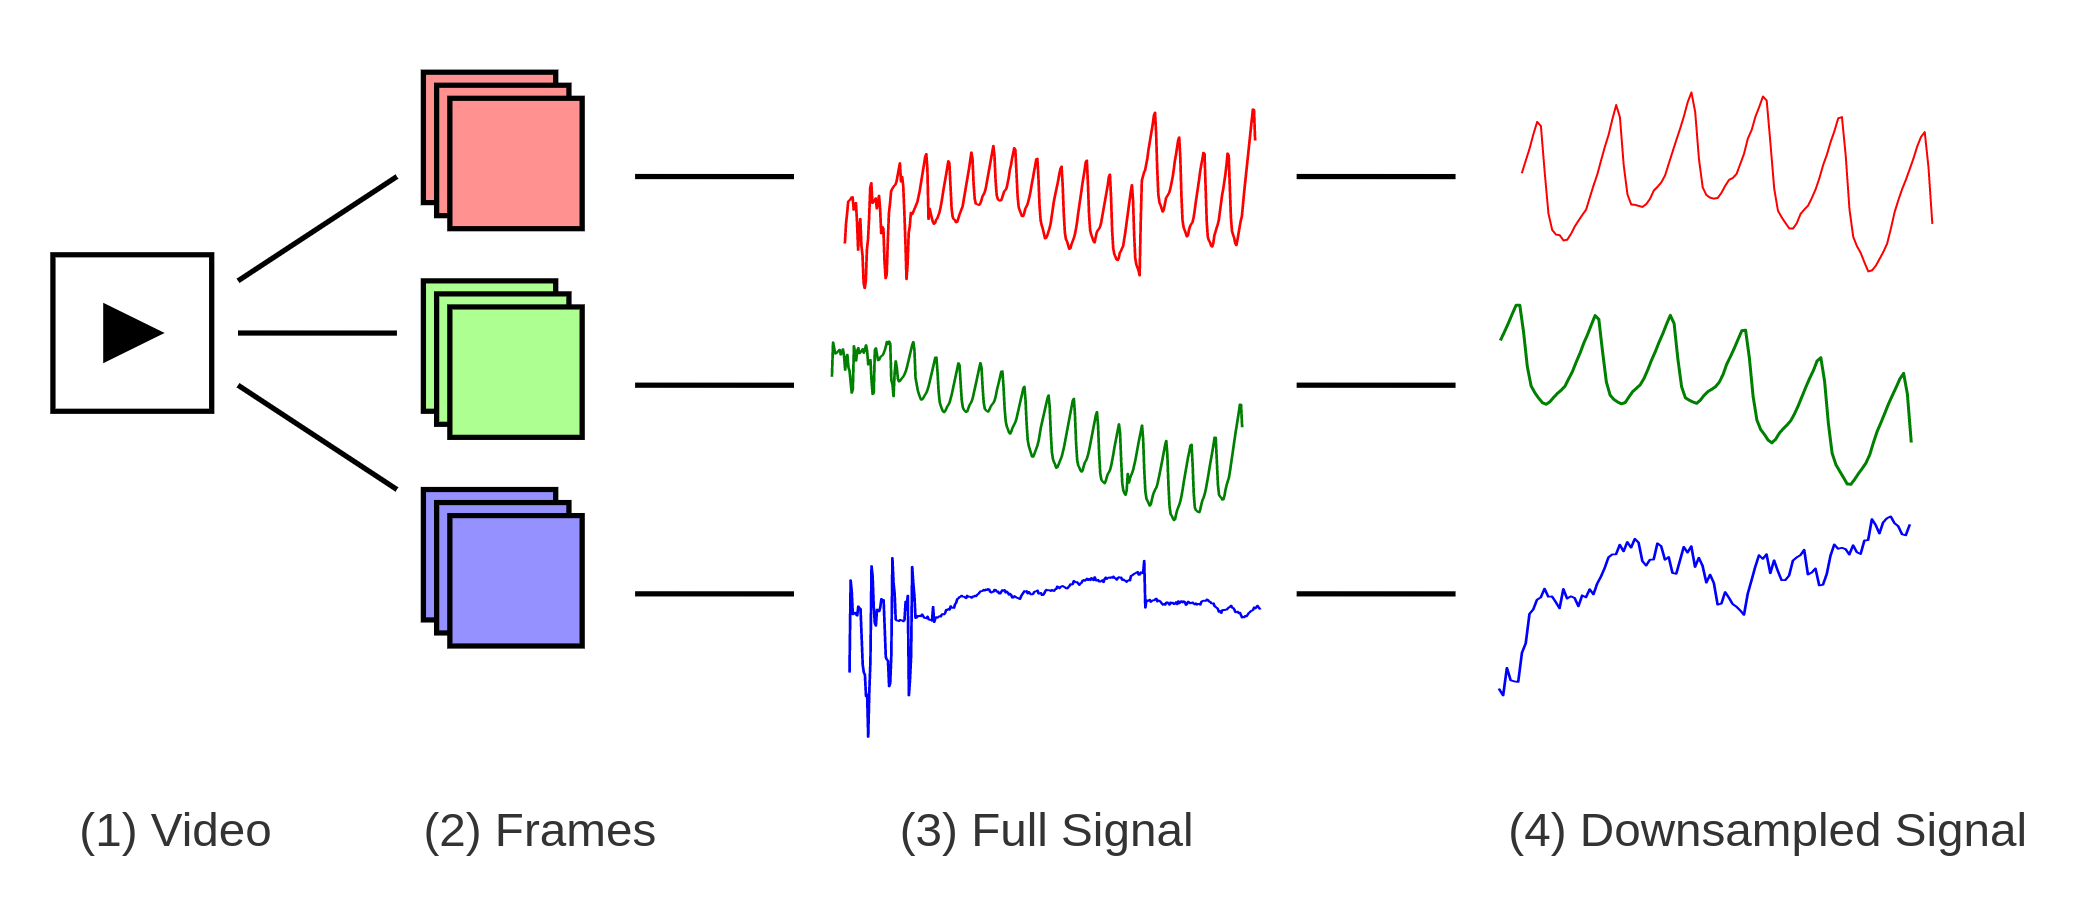
\includegraphics[width=.9\linewidth]{png_images/preporcessing.png}
  \caption{\csentence{Preprocessing steps.}
      An illustration of each step conducted in the preporcessing stage.}
\end{figure}
\FloatBarrier

% TODO: Change description
\subsubsection*{Training}
The preprocessed data trained using deep learning algorithm specifically FCN as
it performs tremendously with the time-series problems including the scaler as
the first layer for normalized input and the global average pooling for
estimating a single value as the final output the model consists of the
constitutional layers show in Fig3.5 trained for 250 epochs with batch size of
32.
\begin{figure}[h!]
  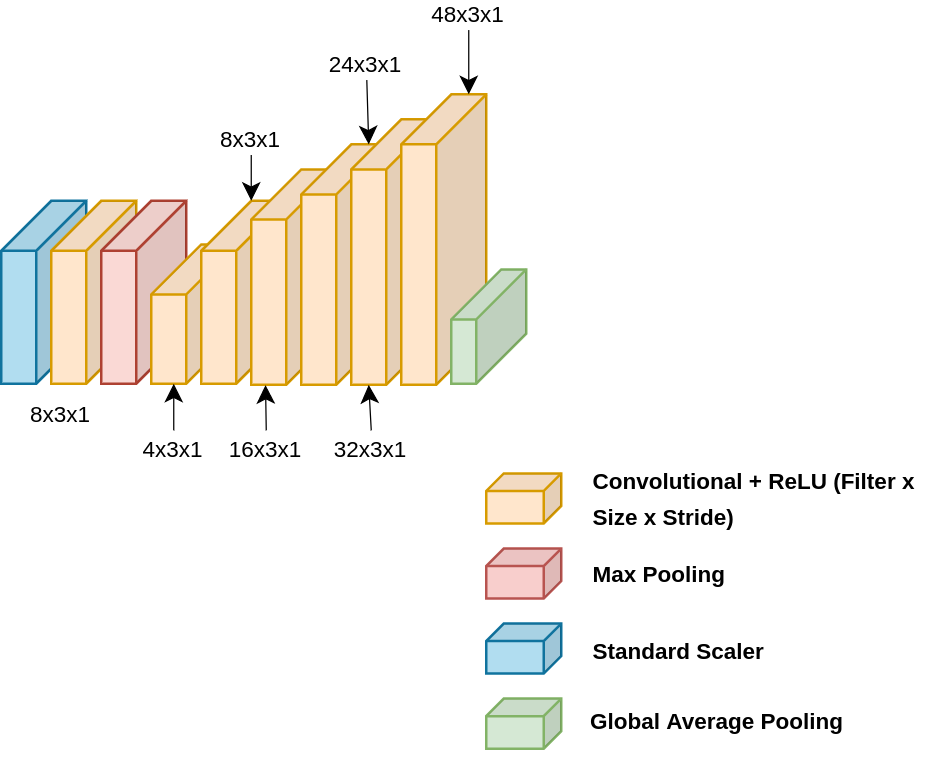
\includegraphics[width=.9\linewidth]{png_images/spo2_model.png}
  \caption{\csentence{FCN model layers.}
  An illustration of the used layers for the FCN deep learning model.}
\end{figure}
\FloatBarrier

% TODO: put the figure

\subsection*{Mobile Application}
The application developed to hub all the major functionality of the system e.g.
collecting the data from the circuit deploying the ML model, calculating the
heart rate using mobile camera, visualizing, storing and sharing users' personal
and medical data through web services.
\subsubsection*{User Interface}
The interface designed to include all the main system functions available to the
user through the main pages ( home – connections – profile) as shown in Figure
3-6, home page includes the ability to connect to the circuit using the upper
plus button, also show all the vital signs measurement  as time series chart to
view the whole day  data, connections page show all the connections and requests
and the upper text field give the user the ability  to send connection request
using email, and profile page gives the user the ability to change all his data.
\begin{figure}[h!]
  \includegraphics[width=.9\linewidth]{png_images/applications_screens.png}
  \caption{\csentence{Application main screens.}
  A screen shot of all the main screen accessable to the user in the application.}
\end{figure}
\FloatBarrier

% TODO: change descritiption
\subsubsection*{Model Deployment}
After training the ML model using Tensorflow Keras the trained model converted
to TfLite file format then the generated file included in the application assets
ready for use, in order to apply the model the user asked to put the index
finger on the main camera and flash as shown in Figure 3-7 for 8 seconds (280
frames) converted from YUV to RGB file format keeping only the mean value of
each channel for each frame, then the 154 middle values of the values are used
as it represent the most stable values for the signal and  to mimic the training
process for accurate results.
% TODO: put the figure
\subsubsection*{Heart Rate Camera Measurement}
Taking into consideration the physical property of light absorption explained
before the Algorithm. (1)  is applied as the mobile camera work on a similar
manner as photo-diode and the flash as the LED for detecting each peak appears
in the heart beat utilizing the collected data in the process of applying the ML
model, however the red channel only used to include the time stamp for each
recorded value then applying Equation (1). 
% TODO: put the figure
\subsubsection*{Handeling User's Data}
After receiving the data from either the Bluetooth interface or internally the
data shown in the screen combined with measurement time as shown in Figure 3-8
then stored in the Firebase real time database which allows near real-time
experience for storing, fetching the data and listen to the data changes from
other devices which allow each user to share his real time data alongside with
other data as shown in Figure 3-8.
\begin{figure}[h!]
  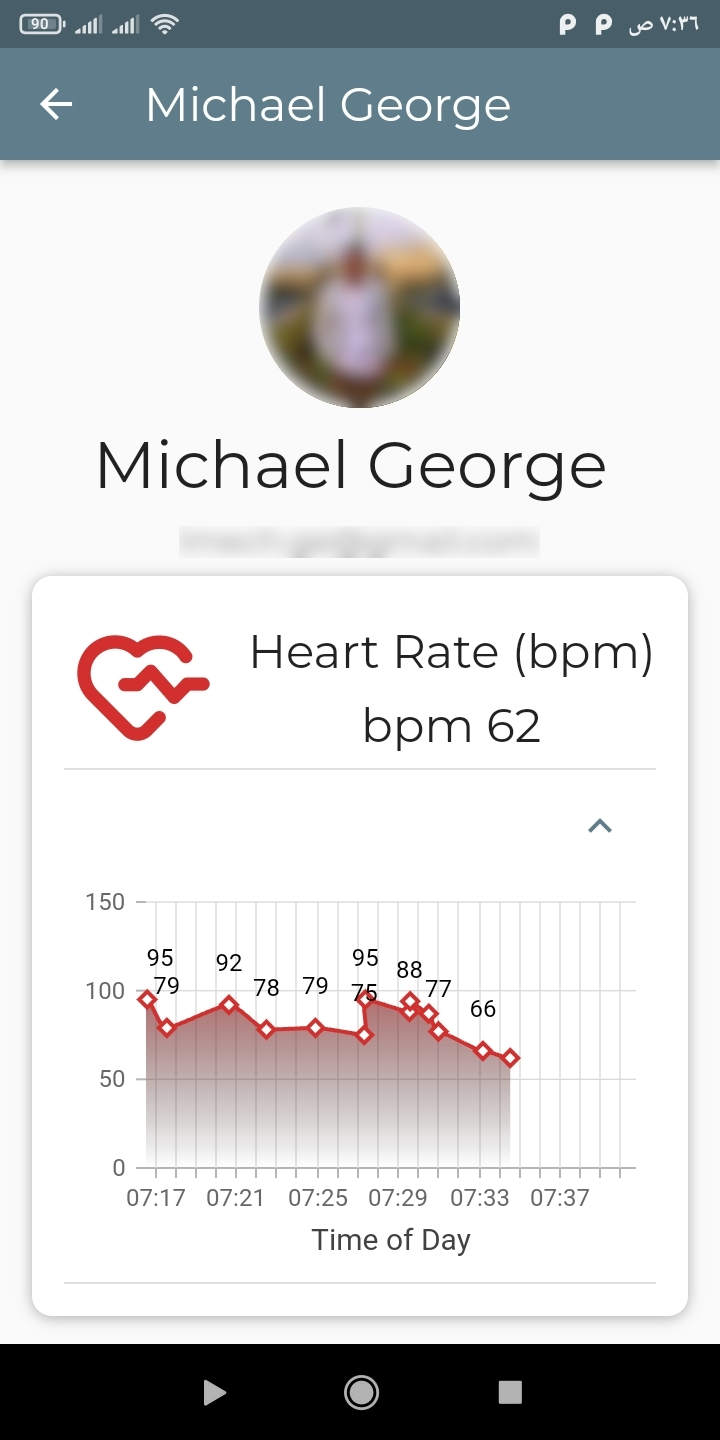
\includegraphics[width=.3\linewidth]{jpg_images/connection_page.jpg}
  \caption{\csentence{Connection page.}
      A screenshots of the connection page from user phone showing all the
      details about the connection.}
\end{figure}
\FloatBarrier

% TODO: put the figure

\subsection*{Cloud Functions}
\subsubsection*{Data Storage}
Due to the extensive amount of collected data from each user giving the
importance for each piece of data, all the collected data stored in the cloud
for backup and for further analysis; Users’ non-sequential data e.g. name, birth
date  stored using Firebase’s “Cloud Firestore Database” service as a key-value
pairs as shown in Figure 3-9 and other users can access the data through email
as key, furthermore the sequential data e.g. heart rate and blood oxygen stored
using Firebase’s “Cloud Real-time Database” for near real time experience for
storing an accessing the data also as key-value pairs and using the measurement
time as key after converting the value to Unix time as shown in Figure 3-10 and
the connections can have a real time monitoring  view of the data by starting a
listener on the user’s document.
% TODO: put the figure
\subsubsection*{Cloud Warnings}
All the received vital signs values compared to the known normal value according
to [b] and classified as normal or abnormal; in case of abnormality the users’
phone automatically sends a notification warning to the users’ phone with a
message of the related abnormal reading as shown in Figure 3-11 and to each of
the connection send a notification warning with the name of the connection and
the related abnormal reading as shown in Figure 3-12.
\begin{figure}[h!]
  \begin{subfigure}{0.45\textwidth}
  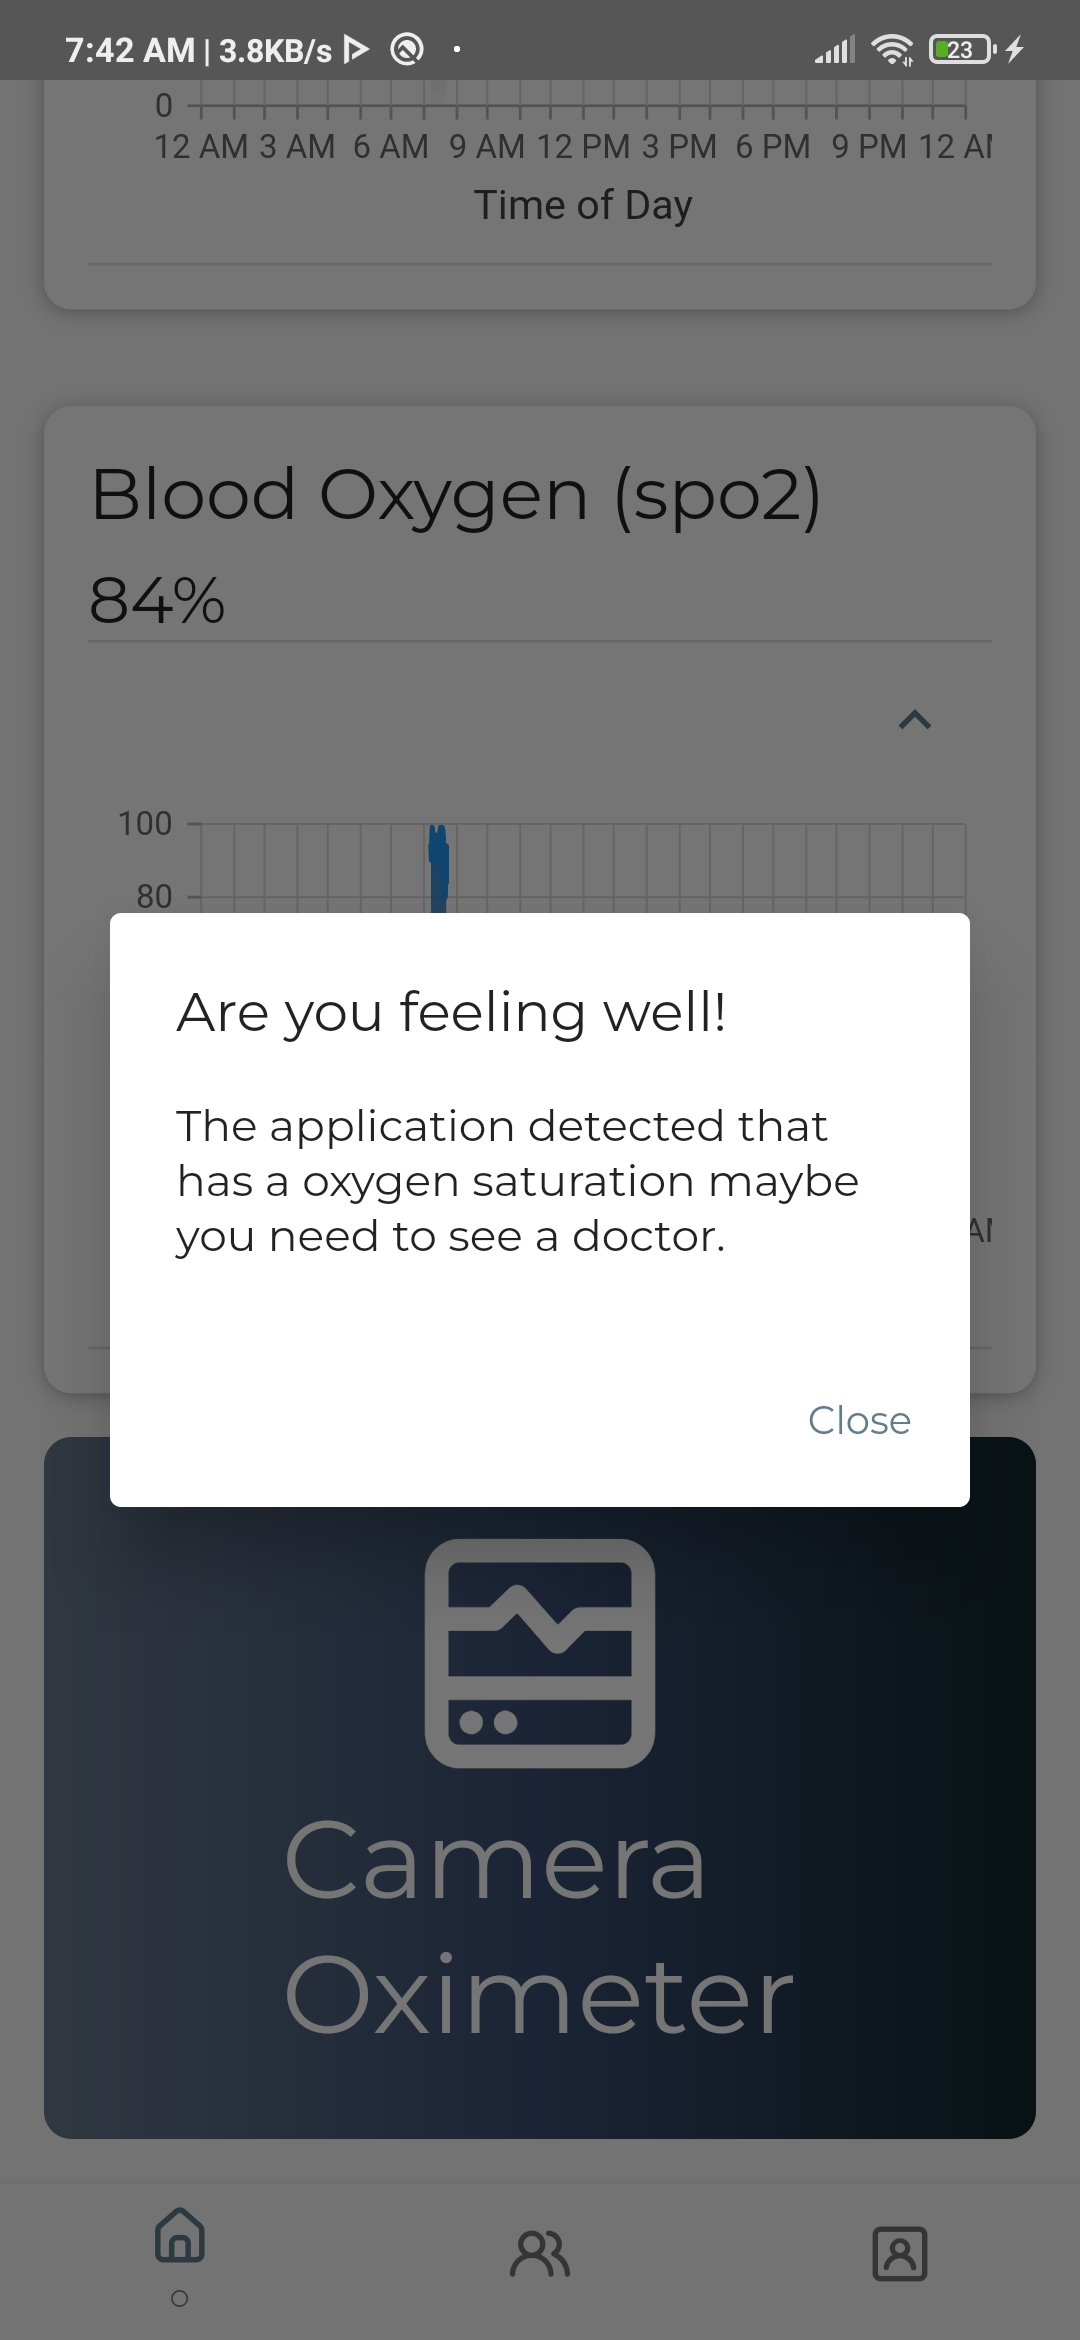
\includegraphics[width=.3\linewidth]{jpg_images/user_warning.jpg}
  \caption{\csentence{User low oxygen saturation warning.}
      A screen shot of the warning appeared to the user after detecting a low
      oxygen saturation case.}
    \end{subfigure}
    \begin{subfigure}{0.45\textwidth}
    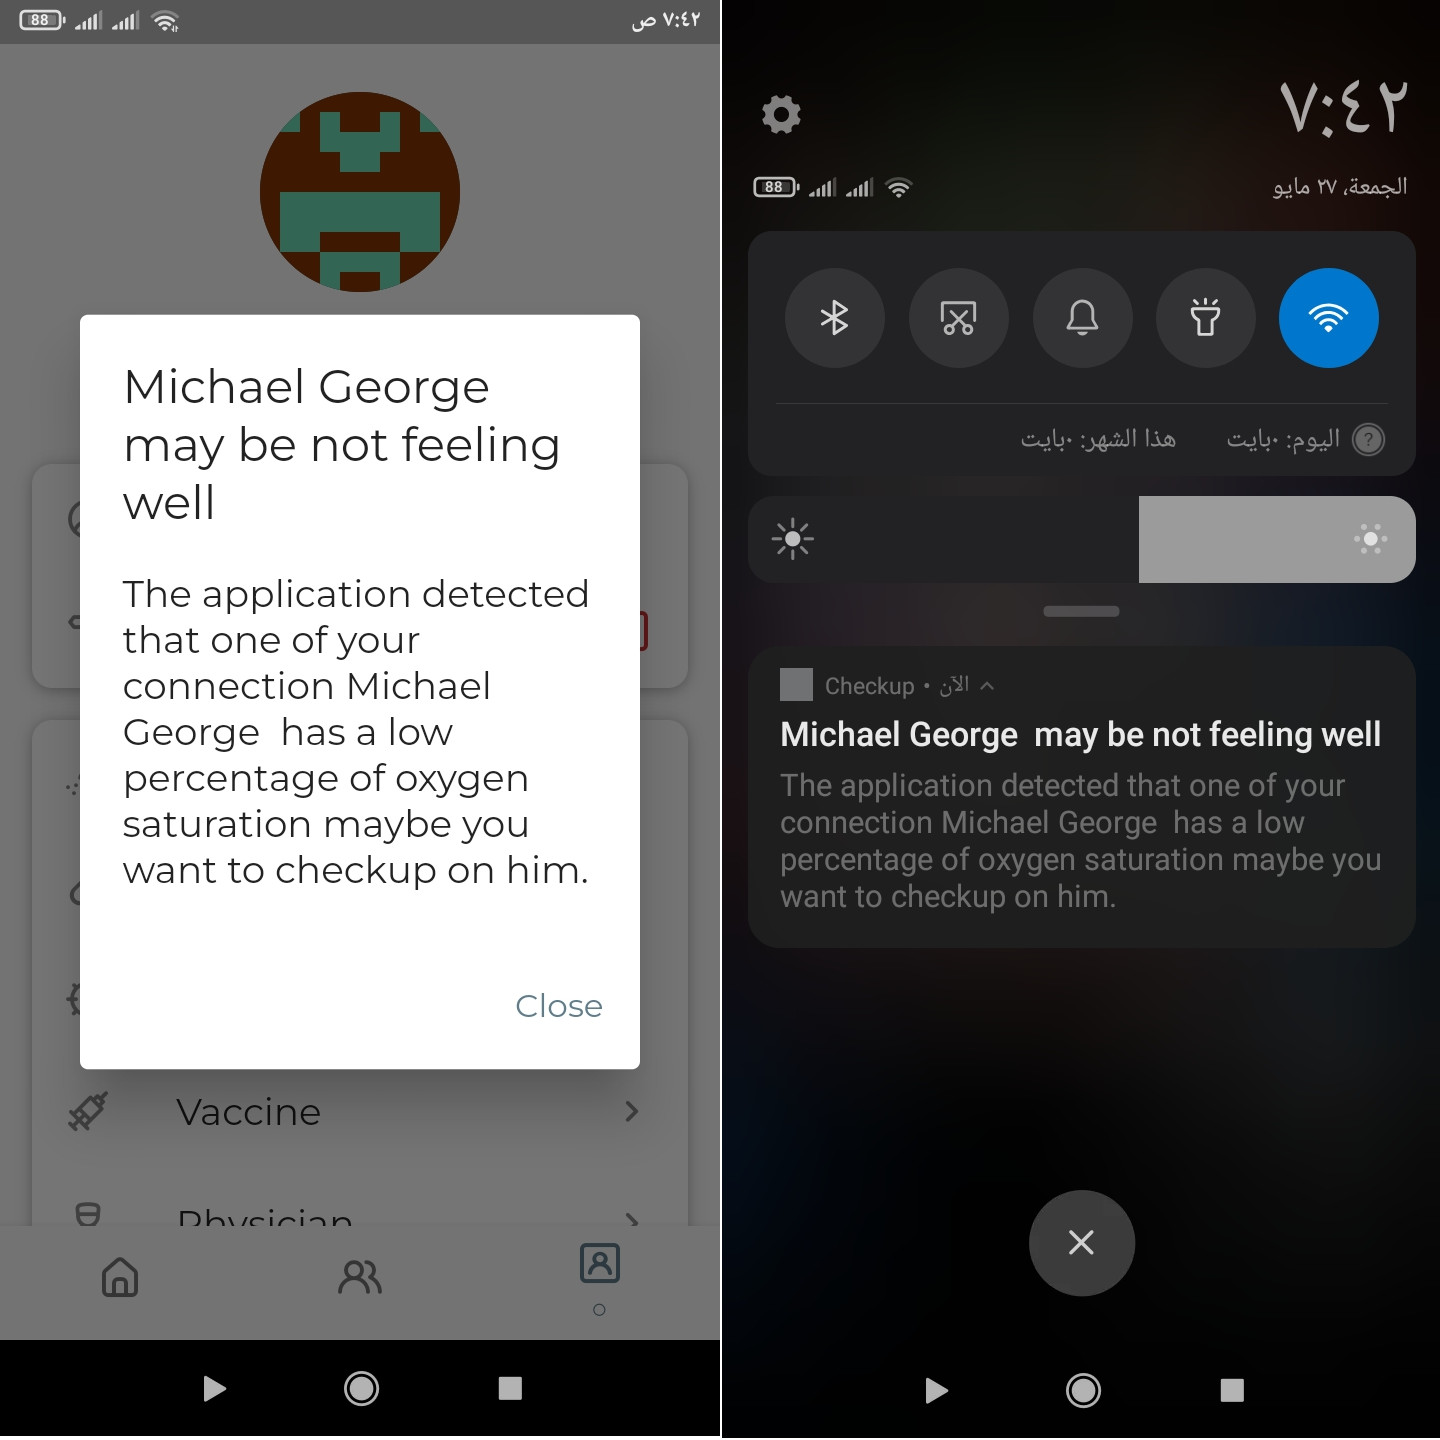
\includegraphics[width=.7\linewidth]{png_images/connection_warnning.png}
  \caption{\csentence{Connection low oxygen saturation warning.}
  A screen shot of the warning appeared to the user after detecting a low
  oxygen saturation case appeared on one of the connections.}
    \end{subfigure}

    \end{figure}
\FloatBarrier

% TODO: put the figure
\subsubsection*{External Gadget Support}
Due to the increasing popularity of the fitness gadget e.g. smart bands and
smart watches, and gadgets ability for making the same measurement with
reasonable accuracy these gadgets can be integrated with the system, but the
closed source nature of the APIs and SDKs with the variant  brand makes it
almost impossible to integrate all the marketed gadget, fortunately most of the
gadgets integrated with Google Fit which provides API for accessing the required
data and more. So, all the gadgets integrated with Google Fit API can be
integrated with the system.
% TODO: put the figure

\section*{Results}
The ML model has achieved an mea of ± 1.9461, using the FCN model on the spo2
signs and the algorithm used in the heart rate achieved unexpected result using
a technique called photoplethysmography (PPG) - is an optically acquired
plethysmogram that may be used to identify changes in blood volume in the
tissue's microvascular bed.\\
We can detect the variability of reflected light and extract the variation of
blood flow by shining a light into a blood irrigated tissue. As we all know,
blood flow is impacted by heart rate, thus we may use blood flow variability to
measure heart rate. The application measures the blood flow volume variability
and displays it in a chart. Now we only need to calculate the heart rate, which
is the frequency of the plotted signal. In our application, we'll use the
phone's camera to shine the camera's flash and measure the power reflected. More
specifically, we'll calculate the average value of the camera image's pixel
intensity. The intensity measured will differ with the blood flow if we cover
the camera and flash with our finger. I used a simple algorithm that measures
the average and the max along our window data, sets the threshold to the mean of
those values, and detects the peaks above that threshold. It then updates the
BPM value with` an attenuation coefficient so we don’t have abrupt changes.\\
The circuit is integrated with our mobile application and it measures the vital
signs every two minutes. The normal ranges of these two vital signs: \\(a) Heart
Rate: 60 to 100 beats per minute [c] \\(b) Blood OxygenSaturation: 95\% or
higher [d] These tables show the real data collected from the GRANZIA pulse
oximeter and our application:
\section*{Tables}
\begin{table}[h!]
\caption{Sample table title. This is where the description of the table should go.}
      \begin{tabular}{cccc}
        \hline
           & Ground Truth  & Predicted & Error Rate\\ \hline
        1 & 94 & 95 & 1\%\\
        2 & 97 & 97 & 0\%\\
        3 & 98 & 99 & 1\%\\
        4 & 99 & 98 & 1\%\\
        5 & 98 & 96 & 2\%\\
        6 & 99 & 99 & 0\%\\
        7 & 99 & 99 & 0\%\\
        8 & 97 & 97 & 0\%\\
        9 & 95 & 97 & 2\%\\
        10& 97 & 97 & 0\%\\
        11& 98 & 99 & 1\%\\
        12& 96 & 99 & 3\%\\
        13& 98 & 99 & 1\%\\ \hline
      \end{tabular}
\end{table}
\section*{Tables}
\begin{table}[h!]
\caption{Sample table title. This is where the description of the table should go.}
      \begin{tabular}{cccc}
        \hline
           & Ground Truth  & Predicted & Error Rate\\ \hline
        1 & 75 & 73  & 2\%\\
        2 & 112& 110 & 2\%\\
        3 & 65 & 68  & 3\%\\
        4 & 78 & 75  & 3\%\\
        5 & 95 & 91  & 4\%\\
        6 & 84 & 82  & 2\%\\
        7 & 70 & 69  & 1\%\\
        8 & 68 & 71  & 3\%\\
        9 & 89 & 90  & 1\%\\
        10& 87 & 87  & 0\%\\
        11& 55 & 53  & 2\%\\
        12& 88 & 91  & 3\%\\
        13& 120& 118 & 2\%\\ \hline
      \end{tabular}
\end{table}
\section*{Conclusion}
This article constructed an IoT-based prototype and applied ML and AI approaches
to the system. The Internet of Things gadget allows for smart monitoring of
human vitals such as oxygen saturation, heart rate, and body temperature.
Real-time ML inference is enabled at the edge to offer essential notifications
to patients as well as the relevant doctors or caregivers in the event that the
patient's vitals show an abnormality. Furthermore, the system is linked to a
live online graphical user interface for both physicians and patients for
management and monitoring. This user-friendly interface securely records and
manages real-time patient data in a secure database. A doctor can simply view
both recorded and live data (including ML inference results) and provide their
analysis accordingly. The system has a number of hardware and software
components.\\
The system comprises of a versatile and user-friendly programme with a nice
interface that can monitor a patient's vitals in real-time without causing
discomfort to the patient. To make rapid and trustworthy judgments locally, the
system employs edge computing techniques. This function reduces latency and
identifies any abnormal situations. The best feature of this programme is that
it can be used on any mobile device that has a camera and a flash.\\
Even from a distance, the patient and guardian can watch the patient's vital
signs. The established system may be proven to be a requirement in the medical
sector, particularly in today's time when people rely heavily on technology and
expect smart solutions to their day-to-day difficulties. The suggested method
not only relieves people from their daily exams, but it also helps the medical
personnel by decreasing their workload and allowing them to handle patients
remotely. This prototype might be utilized at medical camps and places where
established hospitals are scarce. In contrast to traditional healthcare, which
is exclusively available in hospitals, the new paradigm of remotely monitoring
patients using cutting-edge technologies like as IoT and AI is the future of
health care and may assist us in leveraging these technologies and maximizing
their advantages. More sensors, i.e., measured vitals, such as an
electrocardiogram, blood pressure, or respiration rate, can be added as part of
this project's future development. More decision-making elements can be
introduced to the project to identify the likelihood of COVID, especially in the
current condition of COVID. Because the model is simple, it may be used in
conjunction with additional characteristics to develop for a specific illness.
The AI component of the system may be enhanced to provide trend analysis on the
user's data. Because medicine is such a wide subject and various disorders might
have similar symptoms, a model with extremely high precision and accuracy would
be necessary. In addition to the model and the site, the prototype may be
utilized as a main registration step in hospitals, saving medical personnel time
in gathering information and measuring vitals. As a result, it will be an
excellent addition for automating the register system in hospitals. Furthermore,
the concept may be expanded into a remote clinic where patients can select
between continuous monitoring and consulting services. Furthermore, the project
may be marketed by developing and deploying more units in a private or public
hospital for initial testing, and if successful, more units can be created and
deployed. As a result, the produced prototype is adaptable and may serve as a
useful component in a variety of applications.

%%%%%%%%%%%%%%%%%%%%%%%%%%%%%%%%%%%%%%%%%%%%%%
%%                                          %%
%% Backmatter begins here                   %%
%%                                          %%
%%%%%%%%%%%%%%%%%%%%%%%%%%%%%%%%%%%%%%%%%%%%%%

\begin{backmatter}

\section*{Competing interests}
  The authors declare that they have no competing interests.

\section*{Author's contributions}
    Text for this section \ldots

\section*{Acknowledgements}
  Text for this section \ldots
%%%%%%%%%%%%%%%%%%%%%%%%%%%%%%%%%%%%%%%%%%%%%%%%%%%%%%%%%%%%%
%%                  The Bibliography                       %%
%%                                                         %%
%%  Bmc_mathpys.bst  will be used to                       %% %  create a .BBL
%file for submission.                     %% %  After submission of the .TEX
%file,                     %% %  you will be prompted to submit your .BBL file.
%%%
%%                                                         %%
%%                                                         %%
%%  Note that the displayed Bibliography will not          %% %  necessarily be
%rendered by Latex exactly as specified  %% %  in the online Instructions for
%Authors.                %%
%%                                                         %%
%%%%%%%%%%%%%%%%%%%%%%%%%%%%%%%%%%%%%%%%%%%%%%%%%%%%%%%%%%%%%

% if your bibliography is in bibtex format, use those commands:
\bibliographystyle{bmc-mathphys} % Style BST file (bmc-mathphys, vancouver,
spbasic). \bibliography{bmc_article}      % Bibliography file (usually '*.bib' )
% for author-year bibliography (bmc-mathphys or spbasic) a) write to bib file
% (bmc-mathphys only) @settings{label, options="nameyear"} b) uncomment next
% line \nocite{label}

% or include bibliography directly: \begin{thebibliography} \bibitem{b1}
% \end{thebibliography}

%%%%%%%%%%%%%%%%%%%%%%%%%%%%%%%%%%%
%%                               %%
%% Figures                       %%
%%                               %%
%% NB: this is for captions and  %% % Titles. All graphics must be  %% %
%submitted separately and NOT  %% % included in the Tex document  %%
%%                               %%
%%%%%%%%%%%%%%%%%%%%%%%%%%%%%%%%%%%

%%
%% Do not use \listoffigures as most will included as separate files

% \section*{Figures} \begin{figure}[h!]
%   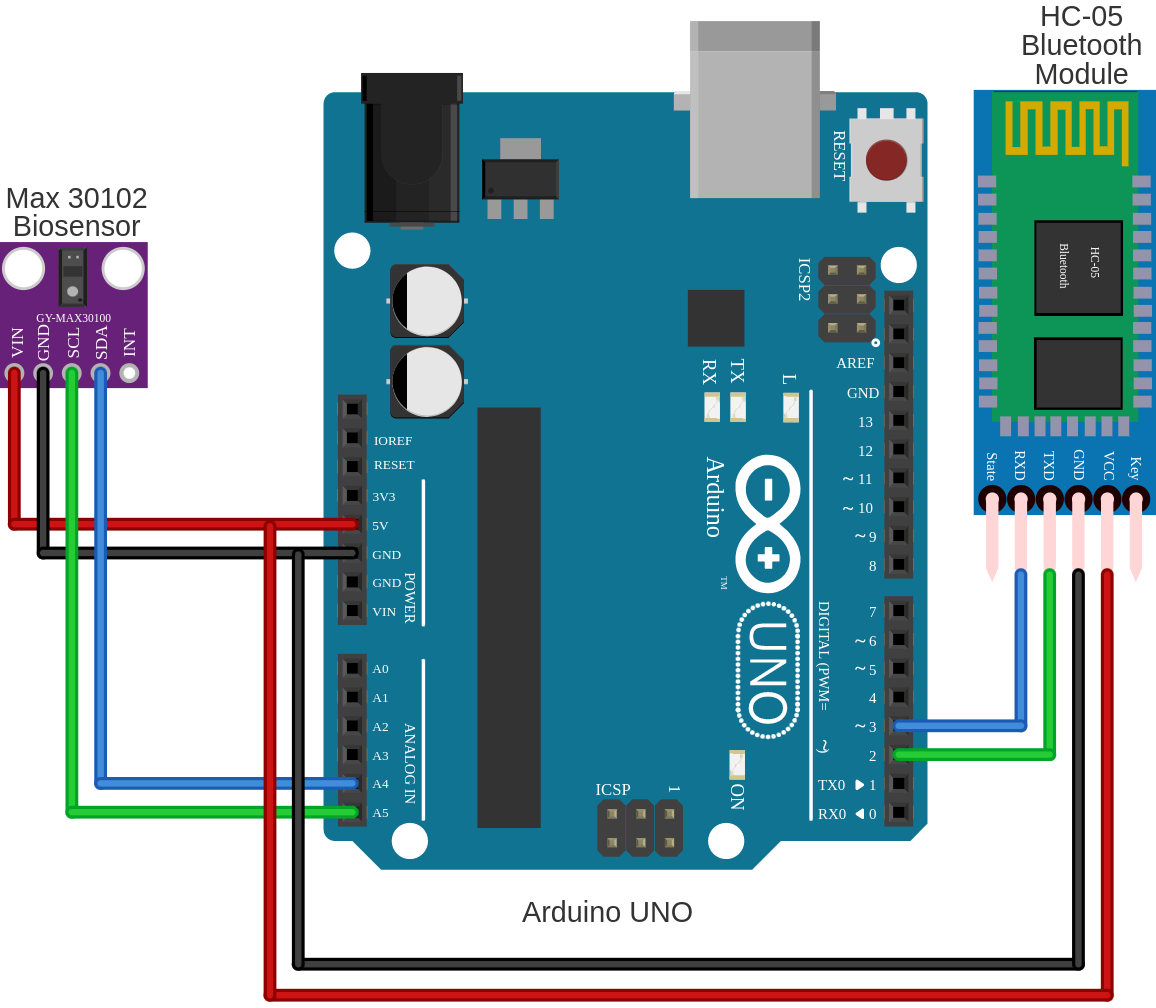
\includegraphics[width=.75\linewidth]{png_images/circuit_desing.png}
%   \caption{\csentence{Sample figure title.} A short description of the figure
%   content should go here.} \end{figure}

% \begin{figure}[h!] \caption{\csentence{Sample figure title.} Figure legend
%   text.} \end{figure}

%%%%%%%%%%%%%%%%%%%%%%%%%%%%%%%%%%%
%%                               %%
%% Tables                        %%
%%                               %%
%%%%%%%%%%%%%%%%%%%%%%%%%%%%%%%%%%%

%% Use of \listoftables is discouraged.
%%
\section*{Tables}
\begin{table}[h!]
\caption{Sample table title. This is where the description of the table should go.}
      \begin{tabular}{cccc}
        \hline
           & B1  &B2   & B3\\ \hline
        A1 & 0.1 & 0.2 & 0.3\\
        A2 & ... & ..  & .\\
        A3 & ..  & .   & .\\ \hline
      \end{tabular}
\end{table}

%%%%%%%%%%%%%%%%%%%%%%%%%%%%%%%%%%%
%%                               %%
%% Additional Files              %%
%%                               %%
%%%%%%%%%%%%%%%%%%%%%%%%%%%%%%%%%%%

\section*{Additional Files}
  \subsection*{Additional file 1 --- Sample additional file title}
    Additional file descriptions text (including details of how to view the
    file, if it is in a non-standard format or the file extension).  This might
    refer to a multi-page table or a figure.

  \subsection*{Additional file 2 --- Sample additional file title}
    Additional file descriptions text.

\end{backmatter}
\end{document}
